\documentclass[10pt,letterpaper]{article} 
\usepackage{toolsper}
%\usepackage{graphicx}‎‎
%\usefonttheme{serif}‎
%\usepackage{ptext}‎
\usepackage{xepersian}
\settextfont{B Nazanin}
\usepackage{lipsum}
\setlength{\parindent}{0pt}
\newcommand{\pf}{$\blacksquare$}
\newcommand{\pic}[2]{
\begin{center}
\includegraphics[width=#2]{#1}
\end{center}
}
\begin{document}
\Large
\begin{center}
به نام خدا

پاسخ تمرینات سری سوم درس آمار و احتمال
\hl
\end{center}
سوال 1) قضیه‌ی دوموآو - لاپلاس اذعان می کند:
\eqn{
\binom{n}{k}p^k(1-p)^{n-k}\approx
{1\over \sqrt{2\pi np(1-p)}}e^{-{(k-np)^2\over 2np(1-p)}}
}{}
هنگامی که $k$ نزدیک به $np$ باشد. در اینجا می خواهیم شهودی از میزان این نزدیکی پیدا کنیم. به ازای $k$ های مختلف داریم:
$$
\begin{cases}
k=1&,\quad \text{\rl{خطای نسبی}}\sim 10^{80}
\\
k=300&,\quad \text{\rl{خطای نسبی}}\approx 7.99
\\
k=490&,\quad \text{\rl{خطای نسبی}}\approx 6.34\times 10^{-5}
\end{cases}
$$
شایان گفتن است که در دو حالت اول، مقدارهای دقیق و تقریبی احتمال تقریبا برابر صفر هستند.
\np
سوال 2)

الف)
$$
\binom{n}{m}\left({M\over N}\right)^m\left(1-{M\over N}\right)^{n-m}
$$
ب)
$$
\binom{M}{m}\binom{N-M}{n-m}\over \binom{N}{n}
$$
ج) در این حالت باید داشته باشیم $n=M+2$ در غیر این صورت احتمال برابر صفر است. با این فرض، پس از تمام شدن گلوله های سفید، حتما دو گلوله‌ی سیاه برداشته خواهند شد و این احتمال برابر یک است.
\eqn{
P&=\Pr[\text{\rl{برداشتن دو سیاه}}|\text{\rl{برداشتن تمام سفیدها}}]
\\&=
{
\Pr[\text{\rl{برداشتن دو سیاه}}\cap\text{\rl{برداشتن تمام سفیدها}}]
\over
\Pr[\text{\rl{برداشتن تمام سفیدها}}]
}
\\&=
{
1
}
}{}
\np
سوال 3) این حالت زمانی رخ می دهد که تعداد قدم زدن های به سمت چپ فرد با تعداد قدم زدن های به سمت راست فرد برابر باشد؛ پس اولین شرط زوج بودن $k$ است در غیر این صورت احتمال برابر صفر خواهد بود. با فرض زوج بودن $k$ داریم:
$$
p=\binom{k}{{k\over2}}[p(1-p)]^{k\over 2}
$$
\np
سوال 4) ابتدا، زیرمجموعه ها را با $A$ و $B$ و سپس پیشامد آن را که عدد $i$ در $A$ و $B$ باشد، به ترتیب با $X_i$ و $Y_i$ نمایش می دهیم. در این صورت احتمال زیر مطلوب است:
\eqn{
\Pr&\{\text{\rl{پیشامد قرار نداشتن عدد 1 در هر دو مجموعه}}
\\&\cap
\text{\rl{پیشامد قرار نداشتن عدد 2 در هر دو مجموعه}}
\\&\cap
\text{\rl{پیشامد قرار نداشتن عدد 3 در هر دو مجموعه}}
\\&\cap
\cdots
\\&\cap
\text{\rl{پیشامد قرار نداشتن عدد $n$ در هر دو مجموعه}}
\}
}{}
به زبان ریاضی:
\eqn{
\Pr\left\{\bigcap_{i=1}^{n} \left[X_i\cap Y_i\right]^c\right\}
}{}
به دلیل استقلال می توان نوشت:
\eqn{
\Pr\left\{\bigcap_{i=1}^{n} \left[X_i\cap Y_i\right]^c\right\}&=
\prod_{i=1}^{n}\Pr\left\{\left[X_i\cap Y_i\right]^c\right\}
\\&=
\prod_{i=1}^{n}1-\Pr\left\{X_i\cap Y_i\right\}
\\&=
\prod_{i=1}^{n}1-\Pr\left\{X_i\}\Pr\{Y_i\right\}
\\&=(1-p^2)^n
}{}
\np
سوال 5) الف) این حالت زمانی ممکن است که تیم $A$ پس از 6 دست، در حداقل 5 دست پیروز شده باشد که این احتمال برابر با احتمال پیروزی در دقیقا 5 دست یا دقیقا 6 دست از 6 دست اول است؛ بنابراین
$$
p=\binom{6}{5}p^5(1-p)+\binom{6}{6}p^6=p^5(6-5p)
$$
ب) 
\eqn{
&\Pr\{
\text{\rl{باخت در حداقل یک دست به تیم $B$}}|\text{\rl{برد تیم $A$}}
\}
\\&=
{
\Pr\{
\text{\rl{باخت در حداقل یک دست به تیم $B$}}\cap\text{\rl{برد تیم $A$}}
\}
\over
\Pr\{
\text{\rl{برد تیم $A$}}
\}
}
}{}
احتمال آن که تیم \lr{A} بازی را ببرد و هیچ دستی را به تیم \lr{B} نبازد برابر $p^9$ است. هم چنین احتمال برد تیم $A$ نیز برابر 
$
\sum_{k=5}^{9}\binom{9}{k}p^k(1-p)^{9-k}
$
 خواهد بود. در نتیجه احتمال مطلوب به شکل زیر محاسبه می‌شود:
$$
1-{p^9\over \sum_{k=5}^{9}\binom{9}{k}p^k(1-p)^{9-k}}
$$
ج) تیم $A$ در صورتی بازی را می برد که حداقل 4 دست از 8 دست باقی مانده را ببرد. این احتمال برابرست با:
$$
{\sum_{k=4}^{8}\binom{8}{k}\over 2^8}\approx 0.6367
$$
\np
سوال 6) احتمال مطلوب عبارتست از:
\eqn{
&\Pr\{
\fa{درست بودن پاسخ تمام دانشجویان}|\fa{یکسان بودن پاسخ تمام دانشجویان}
\}
\\&=
{
\Pr\{
\fa{درست بودن پاسخ تمام دانشجویان}\cap\fa{یکسان بودن پاسخ تمام دانشجویان}
\}
\over
\Pr\{
\fa{یکسان بودن پاسخ تمام دانشجویان}
\}
}
}{}
پیشامد آن که تمام دانشجویان مستقل از هم به پاسخ درست برسند، حالت خاصی از کوشش مکرر و احتمال آن برابر $p^n$ است. احتمال آن که دانشجویان به پاسخ یکسانی برسند طبق قاعده‌ی احتمال کل برابر احتمال پاسخ یکسان در دو حالت پاسخ درست یا نادرست است. احتمال آن که تمام دانشجویان به پاسخ نادرست رسیده باشند برابر $(1-p)^n$ و در نتیجه احتمال مطلوب برابر 
$$
{p^n\over p^n+(1-p)^n}={1\over 1+\left(1-{1\over p}\right)^n}
$$
خواهد بود. نسبت $1-{1\over p}$ را می توان معیاری از سختی سوال ارزیابی کرد. در حقیقت هر چه سوال به تعبیر ریاضی آن ``سخت تر'' باشد، احتمال درست پاسخ دادن تمام دانشجویانی که به پاسخ یکسان رسیده اند کمتر است. به علاوه هر چه تعداد دانشجویان بیشتری پس از امتحان به یک پاسخ رسیده باشند، احتمال آن که همه‌ی آنها اشتباه کنند بیشتر می شود. این وضعیت را می‌توان در نمودار زیر مشاهده کرد:
\begin{center}
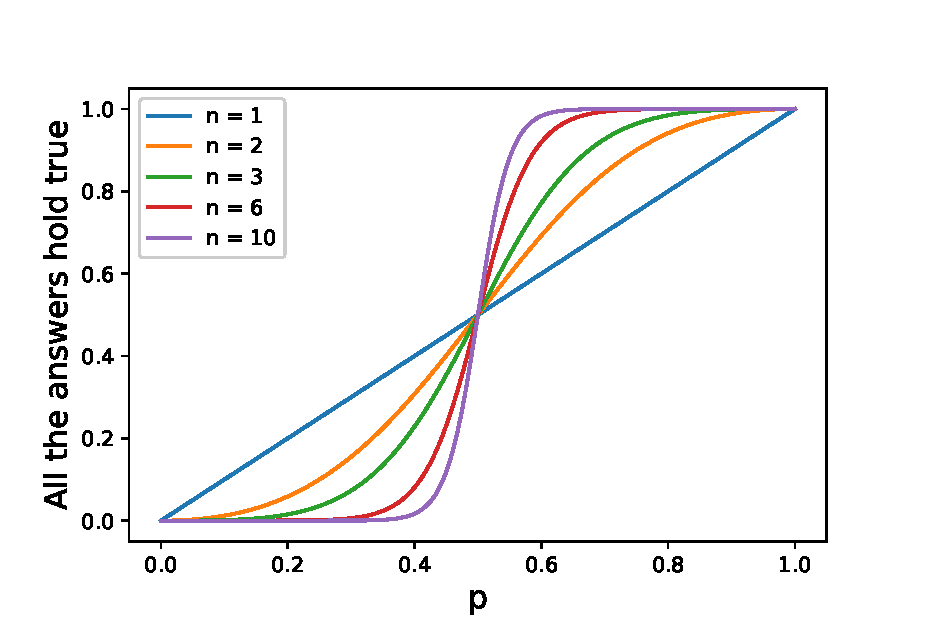
\includegraphics{HW3_Q6.eps}
\end{center}
\end{document}